\documentclass[letterpaper, 12pt]{article}

\usepackage{caption}
\usepackage{float}
\usepackage[T1]{fontenc}
\usepackage[lmargin=1 in, rmargin=1 in, tmargin=1 in, bmargin=1 in]{geometry}
\usepackage{graphicx}
\usepackage{hyperref}
\usepackage{times}
\usepackage{xcolor}

\begin{document}

\textbf{Associate editor}

\bigskip

\textit{In addition to the reviewer's comments, the following references should be cited:
\begin{itemize}
\item L48. Study of LFE has been continuing for about two decades, and it may be difficult to cite all the important previous studies. The review of Beroza and Ide (2011, Annual Rev. Earth Planet. Sci.) covers the first decade.
\item L53. Tremor can be explained as a swarm of LFEs (Shelly et al., 2007, Nature).
\item L56. The source of the tremor and the LFEs is located on the plate boundary (Shelly et al., 2006, Nature; Bostock et al., 2012, G-cubed). Or as a summary by Audet and Kim (2016, Tectonophysics).
\item L58. In addition to the currently cited Ide et al. (2007, GRL), Bostock et al. (2012, G-cubed) and Royer and Bostock (2014, EPSL) are also appropriate for the mechanism study in Cascadia.
\item L63. Obara (2002, Science) should obviously be cited, but is inappropriate as a basis for a correlation study between tectonic tremor and slow slip. Obara et al. (2004, GRL) is better.
\end{itemize}}

\bigskip

We added these references in the text.

\bigskip

\textbf{Reviewer 1}

\bigskip

\textit{Figure 1: Depth contour of subducting plate and surface traces of the San Andreas fault zones (SAF) should be in the figure for easier understanding because authors mentioned about LFE families are on SAF and in the subduction zones (Lines 176 - 183). It should be also helpful to include a figure of depth cross section for LFE hypocenters.}

\bigskip

We added the depth contours of the plate boundary model from McCrory et al. (2006) and fault lines. We added a cross section with the depth of the LFE families.

\bigskip

\textit{Lines 73 - 74: Bostock (2015, https://doi.org/10.1002/2015JB012195) provides 10-year catalog of LFES at the Vancouver Island.}

\bigskip

We added the reference in the text.

\bigskip

\textit{Lines 75 - 76: Japan Meteorological Agency (JMA) provides LFE catalog in Japan since 2004. Kato and Nakagawa (2020, https://doi.org/10.1186/s40623-020-01257-4) also provides LFE catalogs in Japan between 2004 - 2015.}

\bigskip

We added the references in the text.

\bigskip

\textit{Line 138: Why did authors used such a long (1 min) time window for matched filter analysis. I think it is common to use time windows of 5 - 10 seconds around the arrival time at each seismic station (e.g., Shelly et al., 2007, https://doi.org/10.1038/nature05666; Kato and Nakagawa, 2020, https://doi.org/10.1186/s40623-020-01257-4).}

\bigskip

The templates from Plourde et al. (2015) have a low signal-to-noise ratio and generally do not show clear P- and S-wave arrivals, so the 60 seconds window helps be sure it contains the P and S waves. Moreover, the wave arrivals can be located close to the beginning or close to the end of the time window, depending on the LFE family considered. We have chosen to keep the whole one-minute time window to be sure to include both the P- and the S-wave arrivals. The templates obtained using LFE detections from the 2-year-long catalog show clearer P- and S-wave arrivals and we have reduced the length of the time window to 30 seconds on average, depending on the LFE family considered. We have remade the templates using only LFEs that were present in both catalogs (FAME and permanent networks). The wave arrivals are now clearer and, to extend farther in time our catalog, we could reduce the size of the time window by using a different starting time for each station, depending on whether it is close or farther away from the LFE source location. 

\bigskip

\textit{Figure 2: It is helpful to show the value of the detection threshold in this figure.}

\bigskip

We analyzed the seismic data one hour a time. For each hour of data, we assumed that there was an LFE each time the average cross-correlation over all stations and channels is higher than 8 times the median absolute deviation. The threshold is thus different for each hour of data and it is difficult to show its values in the figure.

\bigskip

\textit{Lines 165 - 175: How second thresholds (CC values vs stations numbers) were chosen for each seismic station? If it is done manually, please provide a list of the threshold as the supplementary table. In addition, how many events did this selection step remove from the catalog? (A figure comparing before and after the selection step will be useful.)}

\bigskip

The choice of the threshold is explained in more detail later in the text, when we explain how we cleaned the longer catalog (2004-2011). The main idea is that if an LFE is present both in the 2007-2009 FAME catalog and in the 2004-2011 permanent networks catalog, then it is unlikely to be a false detection. We assumed that all LFEs present in both catalogs are true detections. The LFEs recorded during the period 2007-2009 that are present in only one catalog are then assumed to be false detections. Our goal is to maximize the number of true detections in the filtered catalogs. For the FAME catalog, we then chose a threshold such that at least 50 \% of the LFE detections kept in the FAME catalog after filtering with the threshold, are true detections, that is they are also in the networks catalog. For the networks catalog, we chose a threshold such that at least 50 \% of the LFE detections kept in the networks catalog after filtering with the threshold (and occurring between 2007 and 2009), are true detections, that is they are also in the FAME catalog. There are thus two thresholds per family. The filtering is done such that the product of the cross-correlation for a given LFE by the number of channels recording at the time when the LFE occurred is higher than the threshold. The thresholds chosen for the FAME and the networks catalog are then different because the stations and the quality of the templates are different for both catalogs. For the period 2004-2007 and 2009-2011, we used the same threshold as determined for the period 2007-2009 for the networks catalog. We added in a supplement a table with the values of the thresholds. \\

Our filtering method kept 37 \% of the LFEs for the networks catalog and 16 \% of the LFEs for the FAME catalog. We have added in the supplements figures of the catalogs without filtering the LFEs.

\bigskip

\textit{Lines 204 - 207: How much are two catalogs (the FAME catalog and the network catalog) different originally? As the station density of FAME stations seems to be equivalent to that of permanent stations, I expect two catalogs do not show significant differences. If there are severe differences between two catalogs, detection process and/or event selection procedure needs to be reconsidered. In addition, I think it is also good to show event catalog detected using both FAME stations and permanent stations. Comparing "FAME + network" catalog and the network catalog at the same period, we can evaluate how much the resolution of LFE detection only with the permanent stations becomes worse than that with additional FAME stations. This is important information to evaluate completeness of the LFE catalog in the periods without FAME stations.}

\bigskip

We have computed the catalog with only the FAME stations and the catalog with only the permanent stations. We have not computed a catalog using both FAME and permanent stations. We agree that it would be interesting to compute this third catalog and study how many LFEs are missed when removing the FAME stations, but this is beyond the scope of this paper.

\bigskip

\textit{Line 209: "two thresholds" for what?}

\bigskip

One threshold to filter the 2007-2009 catalog computed with the FAME stations and one threshold to filter the 2004-2011 catalog computed with the permanent stations. We use two different thresholds because the quality of the templates is not the same for the two catalogs.

\bigskip

\textit{Line 215: It will be helpful to visually show temporal changes of the number of available seismic stations.}

\bigskip

We have added two figures in the supplement with number of channels available as a function of time.

\bigskip

\textit{Line 249: Surface wave triggering of LFEs at the Nankai trough was reported in Miyazawa et al. (2008, https://doi.org/10.1186/BF03352858) and references therein before Han et al. (2014).}

\bigskip

We added the reference in the text.

\bigskip

\textit{Lines 271 - 273: Is there no evidence for dynamic triggering as well?}

\bigskip

We did not see any burst of LFEs coincident with the arrival of seismic waves from regional or distant earthquakes.

\bigskip

\textit{Lines 290 - 294: I think the vertical axis of Figure 9 should be average recurrence interval rather than the number of events.}

\bigskip

We changed the figure and plotted recurrence time instead of number of events.

\bigskip

\textit{Line 296: Tidal triggering of tremors was reported in many studies before Houston (2015), including Shelly et al. (2007, https://doi.org/10.1029/2007GC001640) and Houston et al. (2011, https://doi.org/10.1038/ngeo1157).}

\bigskip

We added these references.

\bigskip

\textit{Line 306: Which fault plane did authors assume to calculate tidal stress?}

\bigskip

The fault plane is the plate boundary model of McCrory et al. (2012): McCrory, P. A., Blair, J. L., Waldhauser, F., Oppenheimer, D. H. (2012) Juan de Fuca slab geometry and its relation to Wadati-Benioff zone seismicity. 
Journal of Geophysical Research: Solid Earth, 2012-09, Vol.117 (B9).

\bigskip

\textit{Lines 323 - 324: Is it possible that this negative sensitivity for family A is due to incorrect fault geometry? As family A is located at the southern edge of the subduction zone, fault geometry could be complex, which might be different from the assumed one.}

\bigskip

We tried to relocate family A using new templates obtained from the LFEs present in both the 2007-2009 FAME catalog and the 2004-2011 networks catalog and S minus P within a station times or P-P times between stations. The family may be located 20 to 30 kilometers north or east from the initial location given by Plourde et al. (2015). There is still a great uncertainty on the depth and this family could be much shallower that the plate boundary. It is then possible that the family is located on a nearby crustal fault running west to east. If that is the case, the fault geometry used for the tidal stress calculation is not appropriate and that would explain the negative sensitivity. We added this comment in the text.

\bigskip

\textbf{Reviewer 2}

\bigskip

\textit{The southern-most LFE family is very interesting! I agree with your assessments that the tidal stress modulation and rapid recurrence intervals suggest this family is on a different fault. With that in mind, I find the lack of further discussion about it unsatisfying. Did you try to re-stack and re-locate this family? It would be great if you could. Even if you conclude that you can't get a reliable depth estimate, I would suggest it's worth showing the template waveforms and discussing a few potential source regions, even if it's highly speculative.}

\bigskip

We have remade the templates for both the FAME and the networks stations using the LFEs present in both the 2007-2009 FAME catalog and the 2004-2011 networks catalog. We tried to relocate the family A using S minus P times for single stations or P-P times between stations. The family A would then be located 20-30 kilometers north or east from the initial location. This does not change the pattern of the tidal stress calculations and the negative sensitivity. However, there is a great uncertainty on the depth and this LFE family may be much shallower than the plate boundary. It is possible that it is located on a nearby crustal fault running west to east. In that case, the fault model for the tidal stress calculation is not appropriate.

\begin{figure}[hbt!]
\centering
\noindent\includegraphics[width=10cm, trim={1cm 11cm 6cm 4cm},clip]{figures/map_LFEs_answers.eps}
\caption{Stations used to relocate LFE family A (black triangles). Initial location from Plourde et al. (2015) (red star) and new locations using S-P times and P-P times (green stars). The numbers in parentheses are the corresponding depth. The family could be located on the crustal fault near station ME28.}
\end{figure}

\bigskip

\textit{Line 290 / Figure 9: I'm a bit confused here. The number of LFE events shown on Figure 9 (< 50) are much too small to be total numbers of events, as made clear by the daily event counts in Figure 8... Are these LFE numbers normalized somehow? Please clarify this.} 

\bigskip

To define the number of events, we assume that there is an event each time that there are at least five LFEs during a single day. If two events are separated by less than five days, we assume that this is a single event. We remade the figure to plot average recurrence time instead of number of events.

\bigskip

\textit{Line 22: what does "other" refer to? Not associated with tremor detections?}

\bigskip

We meant other smaller episodes of LFE activity in between the big tremor episodes. We modified this sentence.

\bigskip

\textit{I think the plain-language summary could be more "plain". Even words/phrases like "episodically", "recurrence intervals", "tidal stress sensitivity" could be expressed in  simpler/more-common words. Things like "tectonic tremor", "slow slip" are certainly not familiar to most people, so that's not plain language.}

\bigskip

We modified the plain language summary.

\bigskip

\textit{Line 41: "...recurrence intervals smaller..." $\rightarrow$ shorter recurrence intervals}

\bigskip

We modified this sentence.

\bigskip

\textit{Line 61: "...in a bursty manner." Maybe you can follow this up with a more explicit description of what "bursty" means...something like "tens to hundreds of events in short period, often lasting a few hours"?}

\bigskip

We added a sentence.

\bigskip

\textit{Line 92: "...were located above the plate boundary." We found that they were shallower than the McCrory model, but we actually assumed that this meant the McCrory model was biased deep. A minor rephrase would be good here (even though we might have just been wrong).}

\bigskip

We modified the sentence.

\bigskip

\textit{Figure 1: it would be nice to have the trench, the San Andreas Fault, (+ the Maacama and Bucknell Creek faults?) and/or plate interface contours on this map}

\bigskip

We added plate contours and faults to the map.

\bigskip

\textit{Line 139: "All these preprocessing operations are done with the Python package obspy". I think it is fine to leave this to the acknowledgements if you prefer to shorten here.}

\bigskip

We move this sentence to the acknowledgements.

\bigskip

\textit{Line 151: maybe a reference to that Shelly (2007, Nature) paper is warranted here for the somewhat standard 8*MAD threshold}

\bigskip

We added the reference.

\bigskip

\textit{Line 161: does the 74\% apply to the total number of LFEs (all families)? Or still the 61 families of the previous sentence?}

\bigskip

It applies to the total number of LFEs for all the 66 families. We modified the text

\bigskip

\textit{Line 173: "The threshold is thus different for each LFE family". I'm not sure what you mean here. Is the threshold constant for each family, or does it vary as stations become active/inactive? Is the threshold consistent for a given number of active stations (on that day), or does it vary between templates? Please try to clarify.}

\bigskip

To keep an LFE in the filtered catalog, we require that the product of the cross-correlation by the number of channels recording at that time is higher than a threshold. We thus require a higher cross-correlation value to keep the LFE in the catalog if some stations are inactive. The threshold is different for each LFE family and applied to the stacked cross-correlation over all channels.

\bigskip

\textit{Line 180: "Additionally, one LFE family located on the southern end of the subduction zone has also shorter recurrence intervals than families located farther north, and behaves more similarly to the strike-slip fault families." What locations are you using here? Also, maybe for clarity you can put (40.1N), or whatever the precise latitude is after "...on the southern end". It may be good to specify the depth here too, since it may not be surprising to see frequent bursts if the family is at 45 km depth.}

\bigskip

We use the same locations as Pourde et al. (2015). We have not tried to relocate the families using the new templates. We specified the latitude and depth of the family in the text.

\bigskip

\textit{Line 223: I think it would be nice to quantify the number of shared (between FAME and network catalogs) events, for each family here instead of just saying "...most events seem to be present..."}

\bigskip

We added a sentence.

\bigskip

\textit{Figure 7: Did the Boyarko et al. study include 2004? I found in your discussion that it does not, but I think it's worth repeating this information in the figure caption. Also, the font size is quite tiny here, it would be nice to ensure that there is no text below size 6-7 on any of the figures.}

\bigskip

The Boyarko et al. tremor catalog starts in 2005. That is why we do not show the tremor for the two 2004 LFE events.

\bigskip

\textit{Figure 9: Does the "upper limit of tremor" mean the westward limit?}

\bigskip

Yes, it is the westward limit of the tremor. We modified the caption.

\bigskip

\textit{Line 309: Can you provide references to justify these coefficient values (0.1, 0.5)?}

\bigskip

We took the same values as Houston (2015) for the friction and the Skempton's coefficient.

\bigskip

\textit{Line 312: "We also computed what would be the expected number of LFEs occurring if the tidal stress changes have no influence on LFE activity." It's not clear to me why this (the black lines in Figure 10) varies so dramatically between families, could you explain a bit further?}

\bigskip

%We divided possible values of the Coulomb stress changes into bins and computed the number of hours for which the Coulomb stress change takes values in each bin. As Coulomb stress change often takes small values and rarely takes high values, the expected number of LFEs is higher around 0 and smaller for big negative or positive values. We did not normalize the results, so the expected number of LFEs is proportional to the total number of LFEs occurring for each family. \\

The shape of the black curves are pretty similar for most of the LFE families.  The y-axis scale refers to the histograms and not the theoretical stress so theoretical stress for families D, C4, F, and G1 are pretty similar.  Family A has smaller theoretical stress levels (x axis) and a different shape.  Family B2 is in a transition between A and the other families. These differences may be due to changing slab geometry in the south (Figure 1).

\bigskip

\textit{Supplementary Material: it might be worth repeating the acronym explanations (IRIS, NDEDC) as well as the links to the data sources in this document}

\bigskip

We added the acronym explanations and the reference for the data sources.

\end{document}